\chapter{Resultados Preliminares}

%Es sumamente importante, para esta etapa del proyecto de  tesis,  tener algunos avances iniciales  en cuanto a la experimentación; esto con el fin de  evaluar la factibilidad del trabajo para posteriormente continuar, en el siguiente semestre, con la tesis final. \\

%En el caso que su tesis requiera experimentos, es importante que utilice gráficos y tablas para explicar de manera mas sencilla sus resultados.

\begin{figure}[ht]
  \centering
  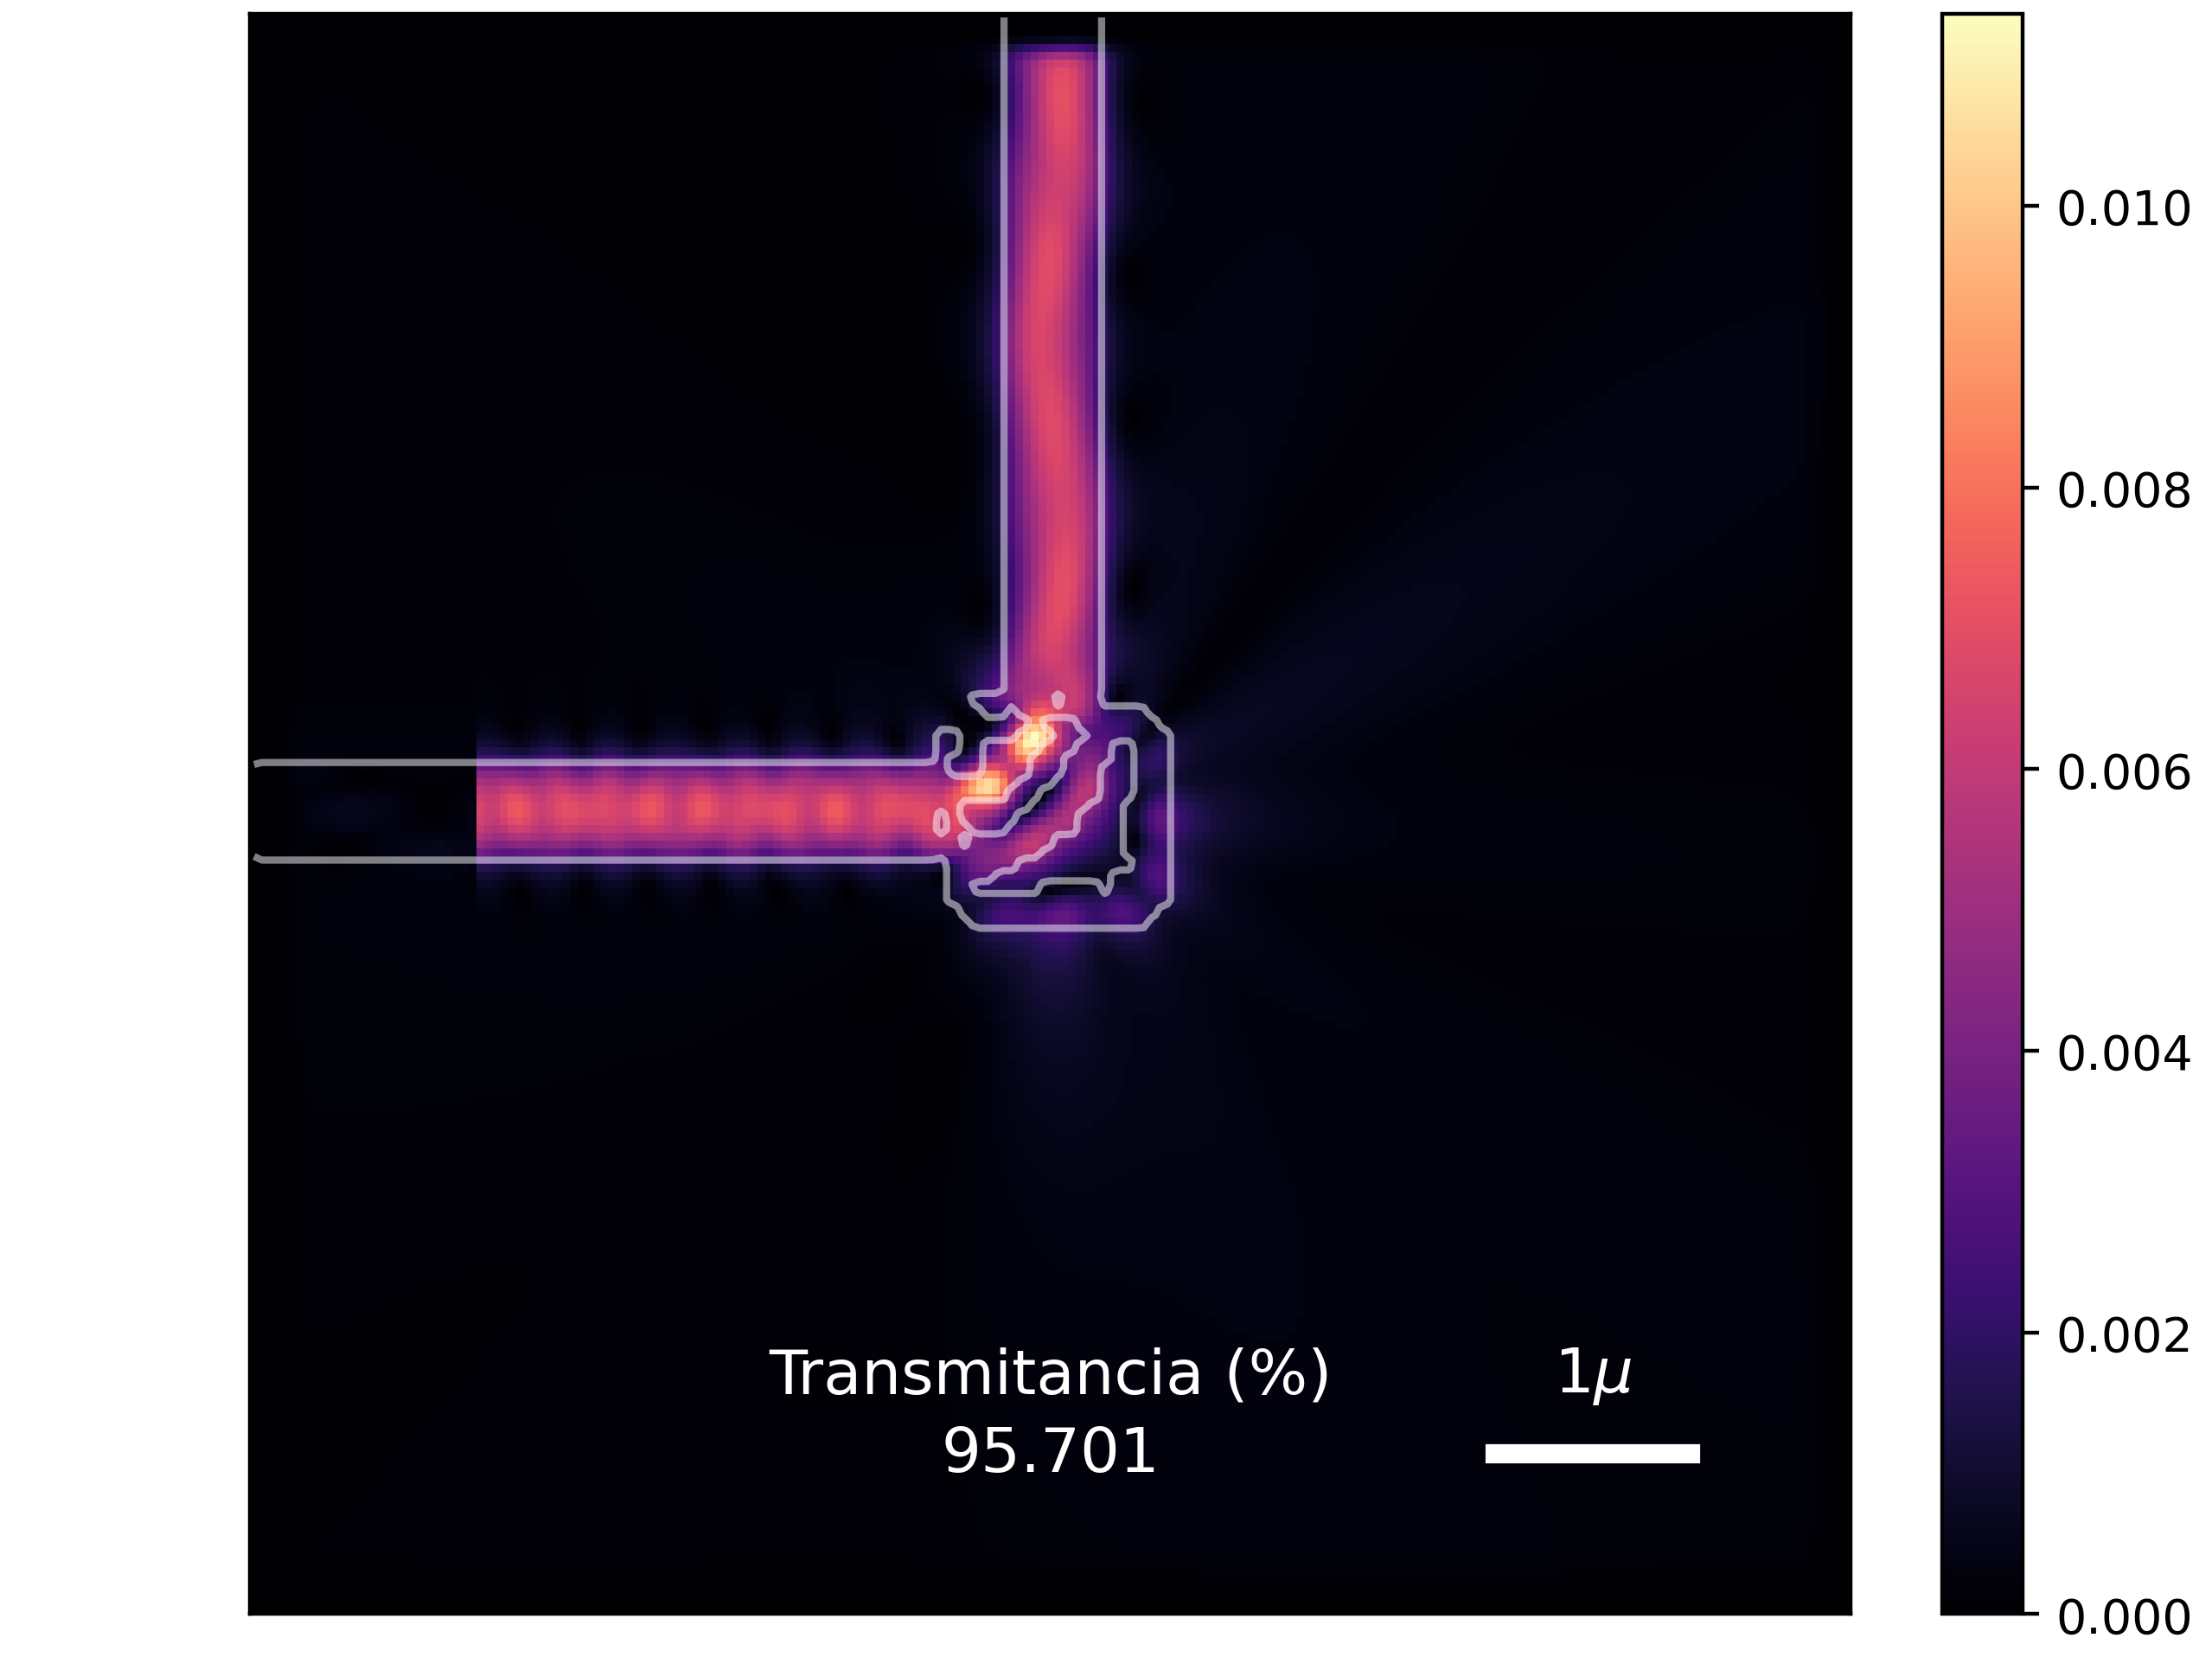
\includegraphics[width=\textwidth]{image/results/device.png}
  \caption{Campo electrico y geometría de un diseño optimizado}
  \label{fig:device}
\end{figure}

Tiempo: 2.788 segundos

Tiempo: 60.543 segundos
